\documentclass{article}
\usepackage{textcomp}
\newcommand{\perthousand}{\textperthousand}
\usepackage{graphicx}
\usepackage{amsmath}
\usepackage{amssymb}
\usepackage{braket}
\usepackage[italicdiff]{physics}
\usepackage{gensymb}
\usepackage{hyperref}
\usepackage[utf8]{inputenc}
\usepackage[T1]{fontenc}
\usepackage{mathtools}
\usepackage[thinc]{esdiff}

\newcommand{\m}[1]{_{\mathrm{#1}}}


\begin{document}

\begin{titlepage}
    \centering
    \vspace*{\fill}

    \vspace*{0.5cm}

    \huge\bfseries
    Oxford Engineering Pre-course Revision Sheets
    \vspace*{0.5cm}

    \large Harik Sodhi

    \vspace*{\fill}
\end{titlepage}
\section{Mathematics}
\subsection{Differentiation}
\begin{enumerate}
    \item $\diff{}{x} 5x^2= 10x$
    \item $\diff{}{x} 4e^x = 4e^x$
    \item $\diff{}{x} 4 \tan{x} = 4 \sec^2{x}$
    \item $\diff{}{x} \sqrt{1+x} = \frac{1}{2\sqrt{1+x}}$
    \item $\diff{}{x} 6 \cos{(x^2)}= -12x \sin{(x^2)}$
    \item $\diff{}{x} e^{3x^4} = 12 x^3 e^{3x^4}$
    \item $\diff{}{x} x^2 \sin{x} = 2x \sin{x} + x^2 \cos{x}$
    \item $\diff{}{x} \frac{\tan{x}}{x} = \frac{x \sec^2{x} - \tan{x}}{x^2}$
    \item $a(t)=\dot{v}(t) = 40t+400 e^{-t} \implies a(2)=80+400 e^{-2} = 134 \text{ ms}^{-2}$. Answer given to 3sf and SI units everywhere are assumed for the units.
    \item $\diff{y}{x}=2xe^{-x} - x^2 e^{-x}=0 \implies x(x-2)=0 \implies x=0 \text{ or } x=2$. Consider that the function is everywhere non-negative, and at $x=0$, it takes the value of $0$, so this is a minima and the other stationary point is a maxima. Therefore, minima at $(0,0)$ and maxima at $(2,4e^{-2})$.
\subsection{Integration}
    \item $\int_{a}^{b} 3x^2 \mathrm{d}x=[x^3]_{a}^{b}=b^3-a^3$
    \item $\int \sin{x} \cos^5{x} \mathrm{d} x= -\frac{1}{6} \cos^6{x} + c$
    \item $\int x^4 + x^3 \mathrm{d} x = \frac{1}{5}x^5 + \frac{1}{4} x^4 + c$
    \item $\int \frac{x}{\sqrt{1-x^2}} \mathrm{d} x=-\sqrt{1-x^2}+c$
    \item $\int_{0}^{2\pi} \sin^2{x} \mathrm{d} x= \int_{0}^{2\pi} \frac{1}{2} - \frac{1}{2}\cos{2x} \mathrm{d} x = [\frac{1}{4}(2x-\sin{2x})]_0^{2\pi}=\pi$
    \item $\int \tan{x} \mathrm{d}x = \int \frac{\sin{x}}{\cos{x}} \mathrm{d} x = -\ln{|\cos{x}|} + c = \ln{|\sec{x}|} + c$
    \item Using $x=\sin{\theta}$, $\mathrm{d} x = \cos{\theta}$, so $\int \frac{1}{\sqrt{1-x^2}} \mathrm{d}x =\int \frac{\cos{\theta}}{\sqrt{1-\sin^2{\theta}}} \mathrm{\theta} = \theta + c = \arcsin{x}+c$
    \item Using $x=a\sin{\theta}$, $\mathrm{d} x = a\cos{\theta}$, so $\int \frac{1}{\sqrt{a^2-x^2}} \mathrm{d}x =\int \frac{a\cos{\theta}}{a\sqrt{1-\sin^2{\theta}}} \mathrm{\theta} = \theta + c = \arcsin{\frac{x}{a}}+c$
    \item $\int x \sin{x} = -x \cos{x} + \int \cos{x} = -x \cos{x} + \sin{x} +c$
    \item $y=0 \implies x(8-x^3)=0 \implies x=0 \text{ or } 2$ so $A=\int_{0}^{2} 8x-x^4 \mathrm{d}x=[4x^2 - \frac{1}{5} x^5]_0^2=16-\frac{32}{5}=\frac{48}{5}$ so the area is $\frac{48}{5}$ units squared.
    \item $x(2)=x(0)+\int_{0}^{2}v(t) \mathrm{d}t = \int_{0}^{2} (20t^2 - 400 e^{-t}) \mathrm{d}t=[\frac{20}{3}t^3+400e^{-t}]_0^2=\frac{160}{3} - 400 (1-e^{-2})= -293 \text{ m}$. So, the particle is $293$ metres from the origin (3sf, assuming SI everywhere).
\subsection{Series}
    \item $10.0 + 11.1 + 12.2 ... + 19.9 = 10 \times \frac{10+19.9}{2}=149.5$
    \item $S_10 = \frac{x(1-(2x)^10)}{1-2x}$
    \item $(a+2x)^n = a^n + 2na^{n-1} x + 2n(n-1) a^{n-2} x^2 + \frac{4}{3} n(n-1)(n-2) a^{n-3} x^3$
\subsection{Functions}
    \item The function is undefined when the denominator is $0$, which means $x=\pm 1$. When approaching $x=-1$ from below, the function goes to to negative infinity. When approaching from above, it goes to positive infinity. When approaching $x=1$ from below, the limit is negative infinity and from above the limit is positive infinity.
\newpage
\subsection{Complex Algebra}
    \item (i) $(1+2i)+(2+3i)=3+5i$ (ii) $(1+2i)(2+3i)=-4+7i$ (iii) $(1+2i)^3=1+6i-12-8i=-11-2i$, (iv) $\arg{(1+2i)}=\atan{2}$ and $\arg{(1+2i)^3}=3\atan{2}-2\pi$ where the last correction is because by convention, $\theta \in [-\pi, \pi]$.
    \item $z \bar{z}= (x+iy)(x-iy)=x^2 + y^2 +xyi - xyi=x^2+y^2$.
    \item $\frac{1+2i}{3+4i} = \frac{(1+2i)(3-4i)}{(3+4i)(3-4i)}=\frac{1}{25} (11+2i)$
    \item $z=\frac{-2\pm \sqrt{4-8}}{2} = -1 \pm i$. When the coefficients of a quadratic are real, the complex solutions are always conjugates
    \item $(\cos{\theta}+i \sin{\theta})^2=(\cos^2{\theta}-\sin^2{\theta})+(2\sin{\theta}\cos{\theta}) i=\cos{2\theta}+i\sin{2 \theta}$
\subsection{Vectors}
    \item This can be done by just dividing by the norm so $\hat{\boldsymbol{v}}=\frac{1}{\sqrt{6}} (\boldsymbol{i}-\boldsymbol{j}+2\boldsymbol{k})$
    \item This can be done by dividing by the norm and then multiplying by $|\vec{OP}|=3$. (i) $\vec{OP}=\sqrt{3}(\boldsymbol{i}+\boldsymbol{j}+\boldsymbol{k})$. (ii) $\vec{OP}=\frac{3}{\sqrt{14}} (\boldsymbol{i}-2\boldsymbol{j}+3\boldsymbol{k})$.
    \item (i) $\boldsymbol{r}=\lambda (\boldsymbol{i}+\boldsymbol{j}+\boldsymbol{k})$. (ii) $\boldsymbol{r}=(\boldsymbol{i}+\boldsymbol{j}+\boldsymbol{k})+\lambda (\boldsymbol{i}-2\boldsymbol{j}+\boldsymbol{k})$.
    \item Suppose the relevant point is $\boldsymbol{r}=\lambda (\boldsymbol{i}+\boldsymbol{j}+\boldsymbol{k})$. The vector from this point to the reference point is $\boldsymbol{r_1}=(\lambda - 3)\boldsymbol{i} + (\lambda-4) \boldsymbol{j}+(\lambda-5)\boldsymbol{k}$. Because the distance is minimal, the dot product with the direction vector of the line is 0. So, $3\lambda-12=0$. So, the point is $(4,4,4)$.
    \item $\cos{\theta}= \frac{10}{\sqrt{14}\times \sqrt{14}}=\frac{5}{7}$ so the angle between them is $\theta = \arccos{\frac{5}{7}}=44.4 \degree$.
    \item This is given by $\boldsymbol{r_1}+\frac{1}{3}(\boldsymbol{r_2}-\boldsymbol{r_1})=\frac{2}{3} \boldsymbol{r_1}+\frac{1}{3} \boldsymbol{r_2}$. So the point required is $(\frac{2x_1+x_2}{3},\frac{2y_1+y_2}{3},\frac{2z_1+z_2}{3})$.
    \item The resultant force is given by $\boldsymbol{f}=3\boldsymbol{i}-\boldsymbol{j}$ and the acceleration takes the same value (adjusting for units) because thebody is unit mass. So, $\boldsymbol{r}(t)=(\frac{3}{2}t^2 + 1)\boldsymbol{i} + (-\frac{1}{2}t^2 +2)\boldsymbol{j}$. For $t>2$, matching the initial velocities: $\boldsymbol{r}(t)=(6(t-2)+1)\boldsymbol{i}+(-\frac{1}{2}t^2 +2)\boldsymbol{j}=(6t-11)\boldsymbol{i}+(-\frac{1}{2}t^2 +2)\boldsymbol{j}$
\end{enumerate}
\newpage
\section{Electricity}
\subsection{Current as a flow of charge}
$I=Anev=\frac{\pi}{4}d^2 nev$, and $t=\frac{l}{v}=\frac{\pi d^2 nel}{4I}=1800 \text{ s}$
\subsection{Resistance and Resistivity}
Total length is given by $L=N \times D_{\text{avg}} \times \pi$, so the resistance is $R=\frac{4\rho N D_{\text{avg}}}{ d^2}=3.4 \text{ }\Omega$
\newline
Power is given by $P=I^2 R = 120 \text{ W}$
\subsection{More resistivity}
Suppose you have $\rho$ for Silver and $x \rho$ for Tin where $x=7.2$. Now consider the perpendicular resistivity. Suppose the specific dimensions are so that if the whole block was Silver, the Resistance would be $R$. Similarly, it would be $xR$ if the block were Tin. Since 2/3 of the block is Tin, the resistance due to Tin is $\frac{2xR}{3}$ and for Silver is $\frac{R}{3}$. Therefore, $\rho_{\perp}=\left(\frac{2}{3}x + \frac{1}{3}\right)\rho$. Now for parallel, using $r$ instead for the same concept as $R$ before, the resistance of the Tin is $\frac{3}{2} xr$ and silver is $3r$ so the effective resistance is $\frac{1}{\frac{1}{3}+\frac{2}{3x}}r$ so $\rho_\parallel = \frac{1}{\frac{1}{3}+\frac{2}{3x}} \rho$ and so the final result is that $\frac{\rho_\perp}{\rho_\parallel}=(\frac{2}{3}x + \frac{1}{3})(\frac{1}{3}+\frac{2}{3x})=\frac{1771}{810}=2.19$
\subsection{Simplified models}
\begin{figure} [h]
    \centering
    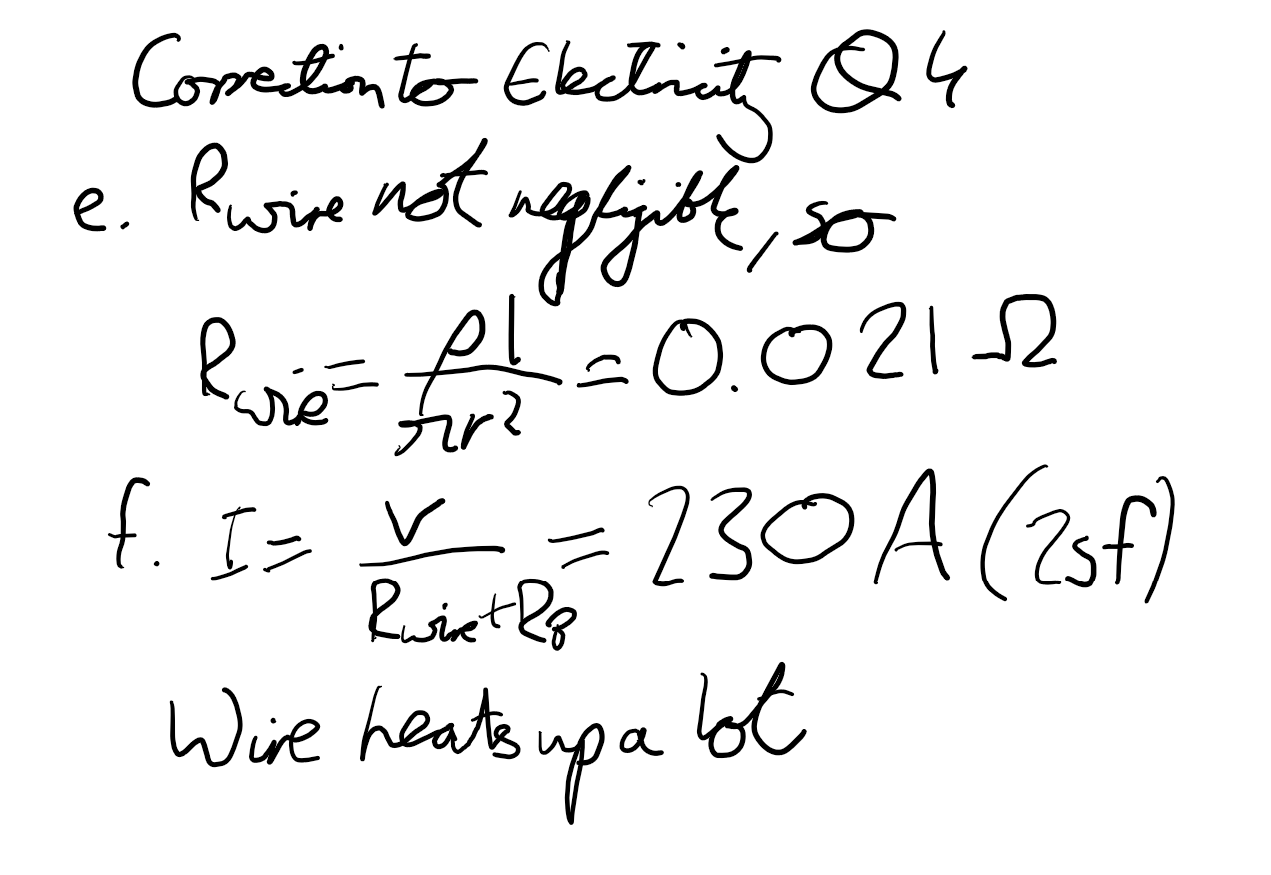
\includegraphics[width=0.8\textwidth]{images/correction.png}
    \caption{Correction to problem 4}
\end{figure}
\end{document}